\documentclass{article}
 

 
\usepackage[margin=1in]{geometry} 
\usepackage{amsmath,amsthm,amssymb}
 \usepackage{graphicx}
 \usepackage{enumerate}
 \usepackage{color}
 \usepackage{hyperref}
 
 \hypersetup{urlcolor=cyan}
 
\newcommand{\N}{\mathbb{N}}
\newcommand{\Z}{\mathbb{Z}}

\newcommand\numberthis{\addtocounter{equation}{1}\tag{\theequation}}

\def\R{\mathbb{R}}
\def\Zp{\mathbb{Z}^+}

\def\a{\alpha}
\def\b{\beta}
\def\c{\gamma}

 
\begin{document}
 
% --------------------------------------------------------------
%                         Start here
% --------------------------------------------------------------
 
 
%%%%%%%%%%%%%%%%%%%%%%%%%%%%%%%%%
% TITLE PAGE
%%%%%%%%%%%%%%%%%%%%%%%%%%%%%%%%% 
\title{
    \textmd{\Huge{Midterm B1}}\\
    \textmd{\huge{Section 4}}
}


\maketitle

Consider the set of points $(-2, 2)$, $(1, 1)$ and $(2, 2)$ and the interpolating polynomial $f(x)$, which is a $2^\text{nd}$ degree polynomial that passes through those points. \\

\textbf{Problem 1} [15pt]: Write down $f(x)$ as a Lagrangian polynomial.

Before anything, I do a quick \textit{qualitative} sketch to see what's going on. \hspace*{3cm}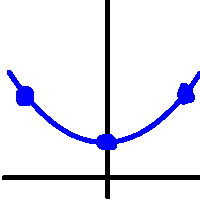
\includegraphics[scale=0.5]{thumbSketch}\\

Since we're told that $f$ is a $2^\text{nd}$ degree polynomial, we know that $f$ is either a parabola, a line, or a point. It's clear from my sketch that it has to be a parabola opening upwards. If that's the case, then for $f(x) = \a x^2 + \b x + \c$, we must have $\a$ strictly greater than $0$. It turns out that this quick analysis will not help us to much for \textit{this} problem, but it never hurts to start with an idea of what's going on. That way, if I end up with something like $\a = -2$ in the end, I'll know that I messed up somewhere. \\

Now that we got that out of the way, let's think of how we write a Lagrangian polynomial when given 3 points. For points $(x_1, y_1)$, $(x_2, y_2)$ and $(x_3, y_3)$, we have the formula \\

\[
f(x)  = y_1 \frac{(x - x_2)(x - x_3)}{(x_1 - x_2)(x_1 - x_3)} + y_2 \frac{(x - x_1)(x - x_3)}{(x_2 - x_1)(x_2 - x_3)} + y_3 \frac{(x - x_1)(x - x_2)}{(x_3 - x_1)(x_3 - x_2)} \numberthis
\] \\

Notice how nicely the "$ - \, x_i $" terms look stacked on top of each other like that. In the first fraction we have $x_2$ right over $x_2$ and the $x_3$ over the $x_3$. The situation is similar for the other two fractions. Also notice that $f$ is a function of $x$. There are two $x$'s in each numerator. Some people made the mistake of substituting point values in for the $x$'s in (1). That's not good. Suppose we didn't have any $x$'s in our expression. Then (1) would just be a sum of constants, giving you some scalar $C$.  You'd have $f(x) = C$, and there's \textit{no way} that $f(x)$ could go through the 3 points I drew horribly up top. \\

Also, notice that our sketch implies that if we multiply out (1) to get some expression $f(x) = \a x^2 + \b x + \c$, then $\a$ better be nonzero and positive. This \textbf{can not} happen if we don't have two $x$'s in the numerators. One other thing to note is that we're given 3 points, and we have 3 expressions in (1). Look at where the $y_1$ and $x_1$'s appear in the first fraction. Look at how similar that is to $y_2$ and the $x_2$'s in the second fraction. \\

Let's take a second to think about how we could generalize (1) a little. That is, suppose we were given four points, $(x_1, y_1)$, $(x_2, y_2)$, $(x_3, y_3)$, and $(x_4, y_4)$ and we want a corresponding Lagrangian polynomial $g(x)$. Without knowing "the formula" for a $4^\text{th}$ order Lagrangian polynomial, I'm just going to set it up the way (1) is set up: \\

\[
g(x)  = y_1 \frac{(x - x_2)(x - x_3)}{(x_1 - x_2)(x_1 - x_3)} + y_2 \frac{(x - x_1)(x - x_3)}{(x_2 - x_1)(x_2 - x_3)} + y_3 \frac{(x - x_1)(x - x_2)}{(x_3 - x_1)(x_3 - x_2)}  + y_4 \frac{(x - ?)(x - ?)}{(x_4 - ?)(x_4 - ?)} 
\] \\

If three points determines a $2^\text{nd}$ order polynomial, it makes sense that four points determine a $3^\text{rd}$ order polynomial. Then we'll need something like this $(x - a)(x- b)(x-c)$ in each numerator. \\

\[
g(x)  = y_1 \frac{(x - x_2)(x - x_3)(x - ?)}{(x_1 - x_2)(x_1 - x_3)} + y_2 \frac{(x - x_1)(x - x_3)(x - ?)}{(x_2 - x_1)(x_2 - x_3)} + y_3 \frac{(x - x_1)(x - x_2)(x - ?)}{(x_3 - x_1)(x_3 - x_2)}  + y_4 \frac{(x - ?)(x - ?)(x - ?)}{(x_4 - ?)(x_4 - ?)} 
\] \\

By analogy, I'm assuming there must also be extra terms in the denominator. Note that the first $x_i$ in each denominator agrees with the $y_i$ in (1). We'll do the same thing here.\\

\[
g(x)  = y_1 \frac{(x - x_2)(x - x_3)(x - ?)}{(x_1 - x_2)(x_1 - x_3)(x_1 - ?)} + y_2 \frac{(x - x_1)(x - x_3)(x - ?)}{(x_2 - x_1)(x_2 - x_3)(x_2 - ?)} + y_3 \frac{(x - x_1)(x - x_2)(x - ?)}{(x_3 - x_1)(x_3 - x_2)(x_3 - ?)}  + y_4 \frac{(x - ?)(x - ?)(x - ?)}{(x_4 - ?)(x_4 - ?)(x_4 - ?)} 
\] \\

Now we just fill in the $?$'s in the obvious way, taking care not to \textit{ever} divide by zero. \textit{Ever}.

\begin{align*}
g(x)  = &y_1 \frac{(x - x_2)(x - x_3)(x - x_4)}{(x_1 - x_2)(x_1 - x_3)(x_1 - x_4)} + y_2 \frac{(x - x_1)(x - x_3)(x - x_4)}{(x_2 - x_1)(x_2 - x_3)(x_2 - x_4)} +  \\
& y_3 \frac{(x - x_1)(x - x_2)(x - x_4)}{(x_3 - x_1)(x_3 - x_2)(x_3 - x_4)}  + y_4 \frac{(x - x_1)(x - x_2)(x - x_3)}{(x_4 - x_1)(x_4 - x_2)(x_4 - x_3)} 
\end{align*}

And we've just blindly derived the general form of a $4^\text{th}$ order Lagrangian polynomial by reason and analogy alone. My point with this is that if you know the formula for a $1^\text{st}$ order Lagrangian polynomial given two points, then you have the resources to figure out the formula for a $2^\text{nd}$ order Lagrangian polynomial, given 3 points. You just have to be a little creative and notice the patterns. \\

Back to the  

\end{document}











































